\chapter{अंतःस्रावी-विज्ञान और समस्थापन}\label{ch:b3:endocrinology}

1921 की गर्मियों में टोरंटो की किसी तपती प्रयोगशाला में दो नौजवानों ने
कुत्तों की अग्न्याशयी नलिकाएँ बाँध दीं, पाचक ऊतक के सूखने की प्रतीक्षा
की, जो बचा उसे पीसा, और वह निष्कर्ष किसी ऐसे कुत्ते में अंतःक्षिप्त
किया जिसे अग्न्याशय निकालकर मधुमेही बना दिया गया था। उसका रक्त-शर्करा
गिर गया। जनवरी तक टोरंटो जनरल अस्पताल में \omterm{def:b3:endocrinology:glucose}{मधुमेह} से मरता कोई
चौदह वर्षीय लड़का वह निष्कर्ष पा रहा था, और हफ़्तों के भीतर वह खा रहा
था, चल रहा था और भार बढ़ा रहा था; वह और तेरह वर्ष जिया। वह पदार्थ,
\omterm{def:b3:endocrinology:glucose}{इंसुलिन}, इक्यावन ऐमीनो अम्लों का कोई पेप्टाइड है, जिसे अग्न्याशय का एक
प्रतिशत रक्त में स्रवित करता है, जहाँ कुछ सौ पिकोमोलर की सांद्रता पर वह
शरीर की हर पेशी और वसा कोशिका को बता देता है कि पिछले भोजन की शर्करा का
क्या करना है। यह अध्याय ऐसे ही संदेशवाहकों के बारे में है: वे क्या हैं,
कोई ऐसी कोशिका, जो उस ग्रंथि से कभी मिली ही नहीं, कैसे जानती है कि उस
संदेश का अर्थ क्या है, वे ग्रंथियाँ स्वयं पुनर्भरण-पाशों की किसी
पदानुक्रमी में कैसे शासित होती हैं, और वह पूरा तंत्र रक्त का ग्लूकोस,
नमक, कैल्सियम तथा तापमान जीवन भर कुछ ही प्रतिशत के भीतर कैसे थामे रहता
है --- और जब कोई एक पाश विफल हो तब चिकित्सालय में क्या होता है।

\section{हॉर्मोन और उनके ग्राही}

\begin{definition}[हॉर्मोन]\label{def:b3:endocrinology:hormone}
\index{हॉर्मोन}\index{अंतःस्रावी ग्रंथि}\index{परास्रावी}\index{स्टेरॉइड हॉर्मोन}\index{पेप्टाइड हॉर्मोन}\index{केंद्रकीय ग्राही}
कोई \emph{हॉर्मोन} ऐसा पदार्थ है जिसे कोई कोशिका रक्त में छोड़ती है और
जो अपना ग्राही ढोती दूर की कोशिकाओं पर काम करता है; कोई
\emph{परास्रावी} संकेत पड़ोसियों पर काम करता है, कोई \emph{स्वस्रावी}
उसी कोशिका पर जिसने उसे बनाया, और कोई तंत्रिका-हॉर्मोन किसी न्यूरॉन
द्वारा रक्त में छोड़ा जाता है। चिरप्रतिष्ठित \emph{अंतःस्रावी
ग्रंथियों} --- \omterm{def:b3:endocrinology:axes}{पीयूष}, अवटु, परावटु, अधिवृक्क, अग्न्याशयी द्वीपिकाएँ,
जननग्रंथियाँ --- के साथ अब हृदय (नैट्रियूरेटिक पेप्टाइड), गुर्दा
(इरिथ्रोपोइटिन), वसा (लेप्टिन), आँत (दर्जन भर पेप्टाइड) और अस्थि भी जुड़
गए हैं। रासायनिक रूप से हॉर्मोन तीन तरह के हैं, और वही रसायन उनका तंत्र
तय कर देता है। \emph{पेप्टाइड तथा प्रोटीन हॉर्मोन} (\omterm{def:b3:endocrinology:glucose}{इंसुलिन}, वृद्धि
हॉर्मोन, \omterm{def:b3:endocrinology:axes}{पीयूष} के हॉर्मोन) राइबोसोमों पर बनते हैं, कणिकाओं में संचित
होते हैं, बहिःकोशिकन से छूटते हैं, प्लाज़्मा में मुक्त चलते हैं,
झिल्लियाँ पार नहीं कर सकते, और कोशिका-पृष्ठ के ग्राहियों पर ---
G-प्रोटीन-युग्मित या काइनेज़-बद्ध --- द्वितीय संदेशवाहकों के ज़रिए
सेकंडों से मिनटों में काम करते हैं; उनके अर्ध-आयु काल मिनटों के हैं।
\emph{स्टेरॉइड} (कॉर्टिसोल, \omterm{def:b3:renal-osmoregulation:controls}{ऐल्डोस्टेरॉन}, एस्ट्रोजन, टेस्टोस्टेरॉन,
और सेकोस्टेरॉइड \omterm{def:b3:endocrinology:calcium}{विटामिन D}) कोलेस्टेरॉल से ज़रूरत के मुताबिक़ बनते हैं,
संचित नहीं होते, वाहक प्रोटीनों से बँधे चलते हैं, झिल्लियाँ पार करते
हैं, और ऐसे \emph{केंद्रकीय ग्राही} बाँधते हैं जो स्वयं अनुलेखन कारक
हैं: उनके असर घंटों में आते हैं और दिनों चलते हैं।
\emph{ऐमीन} दोनों के बीच पड़ते हैं: एड्रिनैलीन सेकंड भर में पृष्ठ पर काम
करता है; और \omterm{prop:b3:endocrinology:thyroid}{अवटु हॉर्मोन}, हालाँकि ऐमीनो-अम्ल व्युत्पन्न हैं,
स्टेरॉइडों की तरह केंद्रकीय ग्राहियों पर काम करते हैं। कोई हॉर्मोन अपने
आप में कुछ नहीं होता: वही एड्रिनैलीन एक वाहिका फैलाता है और दूसरी
सिकोड़ता है, क्योंकि उनकी चिकनी पेशियाँ भिन्न ग्राही-उपप्रकार ढोती हैं,
और वही कॉर्टिसोल यकृत में रक्त-ग्लूकोस चढ़ाता है और किसी \omterm{def:b3:adaptive-immunity:lymphocytes}{लसीकाणु} को दबा
देता है, क्योंकि उन दोनों कोशिकाओं का \omterm{def:b3:chromatin-epigenetics:nucleosome}{क्रोमैटिन} अपने ग्राही को भिन्न
जीन सौंपता है।
\end{definition}

\begin{omfigure}
\begin{tikzpicture}[every node/.style={font=\scriptsize}, >=stealth]
  % peptide pathway
  \draw[thick, omDef, fill=omDef!10] (0,0) rectangle (5.2,3.4);
  \node[above] at (2.6,3.4) {पेप्टाइड या ऐमीन हॉर्मोन --- पृष्ठीय ग्राही};
  \draw[thick, omDef] (0,2.6) -- (5.2,2.6); \node[left, font=\tiny] at (5.2,2.75) {झिल्ली};
  \node[circle, fill=omThm!60, inner sep=2pt, label={[font=\tiny]right:हॉर्मोन}] (h1) at (1.4,3.1) {};
  \draw[thick, omDef!80!black, fill=omDef!40] (1.1,2.3) rectangle (1.7,2.9); \node[below, font=\tiny] at (1.4,2.3) {ग्राही};
  \draw[->, thick] (2.0,2.1) -- (3.0,2.1) node[right, align=left, font=\tiny] {G प्रोटीन या\\काइनेज़ क्रियाशीलता};
  \draw[->, thick] (2.6,1.75) -- (2.6,1.25) node[below, align=center, font=\tiny] {cAMP, Ca$^{2+}$, IP$_3$ या\\फ़ॉस्फ़ोरिलन-शृंखला};
  \draw[->, thick] (2.6,0.55) -- (2.6,0.25) node[below=-2pt, font=\tiny] {एंज़ाइम चालू: सेकंडों से मिनटों में};
  % steroid pathway
  \draw[thick, omProp, fill=omProp!10] (6.4,0) rectangle (11.6,3.4);
  \node[above] at (9.0,3.4) {स्टेरॉइड या अवटु हॉर्मोन --- केंद्रकीय ग्राही};
  \draw[thick, omProp] (6.4,2.6) -- (11.6,2.6);
  \node[circle, fill=omMeth!70, inner sep=2pt, label={[font=\tiny]right:वाहक पर हॉर्मोन}] (h2) at (7.6,3.1) {};
  \draw[->, thick] (7.6,2.95) -- (7.6,2.2) node[below, font=\tiny] {आर-पार विसरित होता है};
  \draw[->, thick] (7.9,1.85) -- (9.0,1.5); \draw[thick, omProp!80!black, fill=omProp!35] (8.8,1.0) rectangle (9.6,1.7); \node[right, align=left, font=\tiny] at (9.65,1.35) {हॉर्मोन--ग्राही\\संकुल, यानी कोई\\अनुलेखन कारक};
  \draw[thick, omProp] (7.0,0.2) rectangle (11.0,0.8); \node[font=\tiny] at (9.0,0.5) {केंद्रक: जीन चालू या बंद --- घंटों से दिनों में};
  \draw[->, thick] (9.2,1.0) -- (9.2,0.82);
\end{tikzpicture}

{\small किसी \omterm{def:b3:endocrinology:hormone}{हॉर्मोन} को सुनने के दो ढंग। जल-घुलनशील \omterm{def:b3:endocrinology:hormone}{हॉर्मोन} पृष्ठ पर ही
रुक जाते हैं और द्वितीय संदेशवाहकों के ज़रिए काम करते हैं, तेज़ और
क्षणिक; लिपिड-घुलनशील भीतर घुसते हैं, ऐसा कोई ग्राही बाँधते हैं जो
अनुलेखन कारक है, और वह कोशिका जो बनाती है उसे बदल देते हैं, धीरे और
देर तक।}
\end{omfigure}

\begin{proposition}[मात्रा और अनुक्रिया]\label{prop:b3:endocrinology:dose}
\index{मात्रा--अनुक्रिया वक्र}\index{अतिरिक्त ग्राही}\index{अधोनियमन}
$R$ ग्राही वाली कोई कोशिका, जिनका वियोजन-अचर $K_{d}$ हो, और जो हॉर्मोन-सांद्रता
$H$ में हो, उनमें से $R\,H/(K_{d} + H)$ अधिकृत रखती है, और अनुक्रिया
प्रायः अधिभोग के साथ किसी लघुगणकीय मात्रा-अक्ष पर किसी सिग्मॉइड के
अनुदिश चढ़ती है, जो किसी ऐसे $\text{EC}_{50}$ पर आधी-अधिकतम होती है जो
प्रायः $K_{d}$ से कहीं नीचे है: कुछ ही प्रतिशत अधिभोग पूरी अनुक्रिया दे
देता है, क्योंकि वह संकेत आगे जाकर प्रवर्धित होता है (एक ग्राही अनेक
G प्रोटीन सक्रिय करता है, एक काइनेज़ अनेक क्रियाधारों का फ़ॉस्फ़ोरिलन
करती है), और वे बचे हुए \emph{\omterm{prop:b3:endocrinology:dose}{अतिरिक्त ग्राही}} उस वक्र को बाईं ओर
खिसका देते हैं तथा उस कोशिका को कम मात्राओं के प्रति संवेदी बना देते
हैं। वह कोशिका अपनी ही संवेदनशीलता साधती है: किसी \omterm{def:b3:endocrinology:hormone}{हॉर्मोन} का लंबा संसर्ग
उसके ग्राही पृष्ठ से हटा देता है (\emph{अधोनियमन}), और यही वह तंत्र है
जिससे लगातार ऊँचा \omterm{def:b3:endocrinology:glucose}{इंसुलिन} \omterm{def:b3:endocrinology:glucose}{इंसुलिन} के अपने असर को कुंद कर देता है; और
वंचन उन्हें बढ़ा देता है। \omterm{def:b3:endocrinology:hormone}{हॉर्मोन} $10^{-12}$ से $10^{-9}$ मोलर पर घूमते
हैं --- यानी अधिकांश उपापचयजों से हज़ार से दस लाख गुना नीचे --- और
इसीलिए ग्राहियों को उन्हें नैनोमोलर बंधुता से बाँधना पड़ता है, और
इसीलिए उन्हें नापने के लिए कोई नई विधि चाहिए थी।
\end{proposition}
\begin{proof}
अधिभोग किसी एकल बंधक स्थल का द्रव्यमान-क्रिया समतापी है। यदि अनुक्रिया
तब संतृप्त हो जाए जब $n \ll R$ ग्राही अधिकृत हों, तो वह तब
आधी-अधिकतम होती है जब $R H/(K_{d} + H) = n/2$, यानी $H = K_{d}\,
(n/2)/(R - n/2) \approx K_{d}\, n/(2R) \ll K_{d}$: यानी EC$_{50}$
ग्राहियों की अधिकता के अनुपात में गिरता है। ग्राही खोने से वह चढ़ जाता
है, और वही उस वक्र पर अधोनियमन का असर है।
\end{proof}

\begin{method}[रेडियो-प्रतिरक्षा परीक्षण]\label{met:b3:endocrinology:ria}
\index{रेडियो-प्रतिरक्षा परीक्षण}\index{प्रतिरक्षा-परीक्षण}
किसी \omterm{def:b3:endocrinology:hormone}{हॉर्मोन} को पिकोमोलर सांद्रता पर नापने के लिए (यालो और बर्सन,
1959): (1) उसके विरुद्ध कोई \omterm{def:b3:adaptive-immunity:antibody}{प्रतिरक्षी} उठाइए; (2) उस \omterm{def:b3:adaptive-immunity:antibody}{प्रतिरक्षी} की कोई
नियत छोटी मात्रा रेडियोसक्रिय रूप से अंकित \omterm{def:b3:endocrinology:hormone}{हॉर्मोन} की किसी नियत मात्रा
से मिलाइए, और वह प्रतिदर्श जोड़िए; (3) उस प्रतिदर्श का अनंकित \omterm{def:b3:endocrinology:hormone}{हॉर्मोन}
\omterm{def:b3:adaptive-immunity:antibody}{प्रतिरक्षी} के स्थलों के लिए अंकित वाले से स्पर्धा करता है, इसलिए वह
प्रतिदर्श जितना अधिक \omterm{def:b3:endocrinology:hormone}{हॉर्मोन} रखेगा उतना ही कम अंक बँधेगा; (4) बँधे और
मुक्त अंक को अलग करके गिनिए; (5) ज्ञात मात्राओं से बने किसी मानक वक्र से
उस प्रतिदर्श की सांद्रता पढ़ लीजिए। उसके वंशज उस समस्थानिक की जगह कोई
एंज़ाइम या कोई प्रतिदीप्तक रखते हैं और विशिष्टता बढ़ाने के लिए दो
\omterm{def:b3:adaptive-immunity:antibody}{प्रतिरक्षी} (कोई ``सैंडविच'') काम में लेते हैं; वे इस अध्याय का हर
\omterm{def:b3:endocrinology:hormone}{हॉर्मोन} रक्त की एक बूँद से नाप लेते हैं, और उन्होंने
अंतःस्रावी-विज्ञान को कोई मात्रात्मक विज्ञान बना दिया।
\end{method}

\section{पदानुक्रमी: अधश्चेतक और पीयूष}

\begin{definition}[अक्ष]\label{def:b3:endocrinology:axes}
\index{अधश्चेतक}\index{पीयूष}\index{द्वारीय तंत्र}\index{मोचक हॉर्मोन}\index{पोषी हॉर्मोन}\index{ऋणात्मक पुनर्भरण}
\emph{अधश्चेतक}, यानी पीयूष के ऊपर मस्तिष्क के कुछ ग्राम, तंत्रिकीय
सूचना --- तनाव, ठंड, दिन की लंबाई, रक्त की \omterm{def:b3:renal-osmoregulation:problem}{परासरणीयता} और ग्लूकोस ---
को हॉर्मोनी आदेशों में बदल देता है। उसकी तंत्रिका-स्रावी कोशिकाएँ
\emph{मोचक \omterm{def:b3:endocrinology:hormone}{हॉर्मोन}} (पेप्टाइड: CRH, TRH, GnRH, GHRH, और निरोधक
सोमैटोस्टैटिन; प्रोलैक्टिन के लिए डोपामीन) वाहिकाओं के किसी निजी
\emph{द्वारीय तंत्र} में छोड़ती हैं, जो उन्हें बिना तनु किए सेंटीमीटर
भर नीचे \emph{अग्र पीयूष} तक ले जाता है, जिसकी कोशिकाएँ
\emph{पोषी \omterm{def:b3:endocrinology:hormone}{हॉर्मोनों}} से उत्तर देती हैं: अधिवृक्क वल्कुट को ACTH, अवटु
को TSH, जननग्रंथियों को LH तथा FSH, यकृत तथा ऊतकों को वृद्धि \omterm{def:b3:endocrinology:hormone}{हॉर्मोन},
और स्तन को प्रोलैक्टिन। लक्ष्य ग्रंथियों के \omterm{def:b3:endocrinology:hormone}{हॉर्मोन} --- कॉर्टिसोल,
थायरॉक्सिन, लिंग-स्टेरॉइड --- पीयूष तथा अधश्चेतक दोनों पर पुनर्भरण
करके अपने ही आदेश बंद करा देते हैं: यानी तीन तहों में
\emph{ऋणात्मक पुनर्भरण}। \emph{पश्च पीयूष} कोई ग्रंथि नहीं, बल्कि
अधश्चेतक के न्यूरॉनों के तंत्रिकाक्ष-सिरे हैं, जो वैसोप्रेसिन तथा
ऑक्सीटोसिन सीधे रक्त में छोड़ते हैं। हर अक्ष की अपनी गतिकी है: अवटु अक्ष
धीमा और स्थिर है, जो वर्षों तक कोई \omterm{thm:b3:endocrinology:loop}{नियत बिंदु} थामे रहता है; अधिवृक्क अक्ष
स्पंदी और दैनिक है, जिसमें कॉर्टिसोल भोर से पहले शिखर छूता है और
घंटे-घंटे झोंकों में स्रवित होता है; और किसी स्त्री का जननग्रंथि-अक्ष
किसी ऐसे धनात्मक पुनर्भरण पर मासिक चक्र चलाता है जो बाकियों में नहीं।
\end{definition}

\begin{omfigure}
\begin{tikzpicture}[every node/.style={font=\scriptsize}, >=stealth]
  \node[draw, thick, rounded corners, fill=omDef!20, align=center, minimum width=3.2cm] (hyp) at (0,3.4) {अधश्चेतक\\CRH, TRH, GnRH, GHRH};
  \node[draw, thick, rounded corners, fill=omDef!20, align=center, minimum width=3.2cm] (pit) at (0,1.7) {अग्र पीयूष\\ACTH, TSH, LH/FSH, GH};
  \node[draw, thick, rounded corners, fill=omProp!25, align=center, minimum width=3.2cm] (gl) at (0,0) {लक्ष्य ग्रंथि\\कॉर्टिसोल, T$_4$, लिंग-स्टेरॉइड};
  \node[draw, thick, rounded corners, fill=omMeth!25, align=center, minimum width=3.2cm] (tis) at (0,-1.7) {ऊतक: असर};
  \draw[->, very thick] (hyp) -- (pit) node[midway, right, font=\tiny] {द्वारीय वाहिकाएँ};
  \draw[->, very thick] (pit) -- (gl) node[midway, right, font=\tiny] {रक्त};
  \draw[->, very thick] (gl) -- (tis);
  \draw[-|, thick, omThm] (gl.west) -- ++(-0.9,0) |- (pit.west) node[pos=0.25, left, font=\tiny, omThm, align=right] {छोटा\\पाश};
  \draw[-|, thick, omThm] (gl.west) ++(-0.9,0) -- ++(-0.7,0) |- (hyp.west) node[pos=0.25, left, font=\tiny, omThm, align=right] {लंबा\\पाश};
  \node[left, align=right, font=\tiny] at (-2.0,4.4) {निवेश: तनाव, ठंड,\\प्रकाश, उपापचयज};
  \draw[->, thick] (-1.9,4.3) -- (hyp.north west);
  % right: the thyroid example with numbers
  \node[right, align=left] at (3.4,3.4) {अवटु अक्ष: TRH $\to$ TSH $\to$ T$_4$, T$_3$;\\T$_4$ का अर्ध-आयु 7 दिन, नियत बिंदु वर्षों थमा;\\मुक्त T$_4$ चढ़ने पर log TSH रैखिक रूप से गिरता है};
  \node[right, align=left] at (3.4,1.7) {अधिवृक्क अक्ष: CRH $\to$ ACTH $\to$ कॉर्टिसोल;\\हर 1--2 घंटे में स्पंद, जागने से पहले शिखर;\\तनाव पुनर्भरण को दरकिनार कर देता है};
  \node[right, align=left] at (3.4,0) {जननग्रंथि अक्ष: GnRH स्पंद $\to$ LH, FSH $\to$\\एस्ट्राडायोल, प्रोजेस्टेरॉन, टेस्टोस्टेरॉन;\\महीने में एक बार धनात्मक-पुनर्भरण का उछाल};
  \node[right, align=left] at (3.4,-1.7) {वृद्धि अक्ष: GHRH, सोमैटोस्टैटिन $\to$ GH $\to$\\यकृत से IGF-1; रात में स्पंद};
\end{tikzpicture}

{\small तीन तहों के अक्ष। \omterm{def:b3:endocrinology:axes}{मोचक हॉर्मोन} द्वारीय वाहिकाओं से होकर \omterm{def:b3:endocrinology:axes}{पीयूष}
तक पहुँचते हैं; \omterm{def:b3:endocrinology:axes}{पीयूष} किसी ग्रंथि को आदेश देता है; और उस ग्रंथि का
\omterm{def:b3:endocrinology:hormone}{हॉर्मोन} ऊपर की दोनों तहें बंद कर देता है। हर अक्ष की अपनी लय है और
अपनी विफलताएँ।}
\end{omfigure}

\begin{proof}[प्रमाण-सामग्री]
बर्टहोल्ड (1849) ने मुर्ग़ों को बधिया किया, जिससे उनकी कलगी, बाँग और
लड़ाकूपन जाते रहे; उनके उदर में कहीं भी, बिना तंत्रिकाओं के, कोई वृषण
फिर से बैठा देने पर वे लौट आए --- यानी वह अंग रक्त के ज़रिए काम करता
था। हैरिस (1950 का दशक) ने चूहों में \omterm{def:b3:endocrinology:axes}{अधश्चेतक} और \omterm{def:b3:endocrinology:axes}{पीयूष} के बीच की
द्वारीय वाहिकाएँ काट दीं: वह \omterm{def:b3:endocrinology:axes}{पीयूष}, जिसकी रक्त-पूर्ति कहीं और से लौटा
दी गई थी, तनाव पर अनुक्रिया देना बंद कर बैठा और अंडाशयों का चक्र थम
गया; गुर्दे के नीचे प्रत्यारोपित कोई \omterm{def:b3:endocrinology:axes}{पीयूष} निष्क्रिय रहा, पर \omterm{def:b3:endocrinology:axes}{अधश्चेतक}
के नीचे, जहाँ द्वारीय वाहिकाएँ फिर उसमें उग आईं, वह काम करने लगा ---
यानी मस्तिष्क उस ग्रंथि पर रक्त-वाहित कारकों से शासन करता है, और फिर
गिलमैन तथा शैली ने उनमें से पहला, TRH, भेड़ों और सूअरों के लाखों
अधश्चेतकों से अलग किया (1969): तीन ऐमीनो अम्ल।
\end{proof}

\begin{proposition}[पुनर्भरण और लघु-रैखिक अवटु]\label{prop:b3:endocrinology:thyroid}
\index{अवटु हॉर्मोन}\index{TSH}\index{अवटु-अल्पता}\index{अवटु-अतिता}\index{घेंघा}
अवटु आयोडाइड भीतर लेती है और थायरॉक्सिन T$_{4}$ (चार आयोडीन) बनाती है,
जिसे ऊतक सक्रिय T$_{3}$ में बदल देते हैं; दोनों लगभग हर कोशिका की
उपापचयी दर चढ़ाते हैं, हृद्-दर तय करते हैं, और जन्म से पहले तथा बाद
मस्तिष्क के परिवर्धन के लिए ज़रूरी हैं। \omterm{def:b3:endocrinology:axes}{पीयूष} का TSH उस ग्रंथि का
संश्लेषण तथा वृद्धि, दोनों चलाता है; और T$_{4}$
TSH को दबाता है। स्थायी अवस्था पर यह संबंध \emph{लघु-रैखिक} है: TSH का
लघुगणक मुक्त T$_{4}$ के अनुपात में गिरता है,
\[
\text{TSH} = \text{TSH}_{0}\,\mathrm{e}^{-\kappa\,(T_{4} - T_{4,0})},
\]
इसलिए मुक्त T$_{4}$ का तिहाई गिरना TSH को लगभग दस गुना चढ़ा देता है ---
और इसीलिए संवेदी जाँच TSH है, T$_{4}$ नहीं: जो ग्रंथि विफल होने लगी हो
वह ऐसा T$_{4}$ दिखाती है जो सामान्य है, पर उसे पहले से कई गुना ऊँचा
कोई TSH थामे है। उस ग्रंथि की विफलता (स्वप्रतिरक्षी विनाश, आयोडीन की
कमी) \emph{अवटु-अल्पता} देती है --- ठंडा, धीमा, थका, ऊँचे TSH के साथ,
और आयोडीन की कमी में उस TSH से बढ़कर \emph{घेंघा} बनी कोई ग्रंथि, जिससे
वह TSH उत्पादन करा ही नहीं पाता; और कोई ऐसा \omterm{def:b3:adaptive-immunity:antibody}{प्रतिरक्षी}, जो TSH की नकल
करे, \emph{अवटु-अतिता} (ग्रेव्स रोग) देता है, जिसमें रोगी गरम, तेज़ और
दुबला होता है और TSH शून्य तक दबा, क्योंकि वह उद्दीपन उस पुनर्भरण से
बच निकलता है। जिस नवजात में \omterm{prop:b3:endocrinology:thyroid}{अवटु हॉर्मोन} न हो उसमें महीनों के भीतर
अपरिवर्तनीय बौद्धिक अक्षमता पनप जाती है, और इसीलिए हर नवजात का TSH रक्त
की एक बूँद पर नापा जाता है।
\end{proposition}
\begin{proof}
\omterm{def:b3:endocrinology:axes}{पीयूष} कोशिका का TSH-निर्गम T$_{3}$ द्वारा ग्राही-अधिभोग पर अनुक्रिया
देता है, और वह स्वयं T$_{4}$ के समानुपाती है, और अधिभोग के किसी बदलाव
पर किसी अनुलेखनी दमन की अनुक्रिया गुणात्मक होती है --- \omterm{def:b3:endocrinology:hormone}{हॉर्मोन} की हर
वृद्धि जो बचा है उसका वही अंश दबाती है --- इसलिए
$\mathrm{d}\ln\text{TSH}/\mathrm{d}T_{4} = -\kappa$, जिससे वह चरघातांक
निकलता है। $\kappa$ को ऐसे फिट किया जाए कि $T_{4}$ का $15$ से
\qty{10}{pmol/L} तक गिरना TSH को $1.5$ से \qty{15}{mU/L} तक चढ़ा दे, तो
$\kappa = \ln 10/5 = \qty{0.46}{L/pmol}$: यानी T$_{4}$ के हर
\qty{1.5}{pmol/L} खोने पर TSH दुगुना हो जाता है, और यही वह प्रवर्धन है
जो उसे संवेदी जाँच बनाता है।
\end{proof}

\begin{omfigure}
\begin{tikzpicture}
\begin{semilogyaxis}[
  width=0.6\linewidth, height=5.6cm,
  axis x line=bottom, axis y line=left,
  xmin=4, xmax=30, ymin=0.02, ymax=200,
  xlabel={मुक्त T$_4$ (pmol/L)}, ylabel={TSH (mU/L)},
  xlabel style={font=\small, at={(axis description cs:0.5,-0.12)}, anchor=north}, ylabel style={font=\small},
  tick label style={font=\small}, xtick={5,10,15,20,25,30}, ytick={0.1,1,10,100},
  yticklabels={0.1,1,10,100},
  clip=false,
]
\addplot[very thick, omDef, domain=4.5:24.4, samples=60] {1.5*exp(-0.46*(x-15))};
\fill[omProp, opacity=0.15] (axis cs:10,0.4) rectangle (axis cs:20,4);
\node[font=\scriptsize, omProp!80!black, anchor=south] at (axis cs:15,4.2) {संदर्भ परास};
\node[font=\scriptsize, omThm, anchor=north west, align=left] at (axis cs:12,150) {विफल होती ग्रंथि:\\TSH ऊँचा, T$_4$ अब भी सामान्य};
\node[font=\scriptsize, omMeth!70!black, anchor=south west, align=left] at (axis cs:22,0.5) {ग्रेव्स रोग:\\T$_4$ ऊँचा, TSH दबा हुआ};
\end{semilogyaxis}
\end{tikzpicture}

{\small अवटु का \omterm{thm:b3:endocrinology:loop}{नियत बिंदु} बाहर से देखा हुआ। चूँकि log TSH, T$_4$ के
साथ रैखिक रूप से गिरता है, उस \omterm{def:b3:endocrinology:hormone}{हॉर्मोन} की कोई छोटी गिरावट उस आदेश की
कोई बड़ी बढ़त पैदा कर देती है --- \omterm{def:b3:endocrinology:axes}{पीयूष} उस ग्रंथि की विफलता का कोई
लघुगणकीय प्रवर्धक है।}
\end{omfigure}

\begin{example}[कॉर्टिसोल: तनाव का अक्ष]\label{ex:b3:endocrinology:cortisol}
कॉर्टिसोल, जो ACTH के तहत अधिवृक्क वल्कुट से आता है, ईंधन लामबंद करता
है (यकृत से ग्लूकोस, पेशी से ऐमीनो अम्ल, वसा से वसा अम्ल), वाहिकाओं को
एड्रिनैलीन के प्रति संवेदी बनाता है, और \omterm{def:b3:innate-immunity:inflammation}{शोथ} तथा प्रतिरक्षा-अनुक्रिया
दबाता है --- और इसीलिए उसके संश्लेषित नातेदार सबसे आम प्रति-शोथ औषधें
हैं। उसकी लय वह घड़ी तय करती है: सुबह 8 बजे \qty{500}{nmol/L}, आधी रात
को उसका पाँचवाँ भाग, और बीच भर घंटे-दो घंटे पर स्पंद, क्योंकि \omterm{def:b3:endocrinology:axes}{अधश्चेतक}
की CRH न्यूरॉन झोंकों में दगती हैं। तनाव --- रक्तस्राव, संक्रमण,
शल्यक्रिया, भय --- उसे मिनटों में दस गुना चढ़ा देता है, और उस पुनर्भरण
को दरकिनार कर देता है। बहुत कम (ऐडिसन रोग, अधिवृक्क वल्कुट का विनाश)
दुर्बलता, कम रक्तचाप, कम ग्लूकोस, और तनाव में ढहना तथा मृत्यु देता है,
जब तक उसकी भरपाई न की जाए; बहुत अधिक (कुशिंग संलक्षण: ACTH बनाता कोई
\omterm{def:b3:endocrinology:axes}{पीयूष} \omterm{def:b3:cancer-biology:hallmarks}{अर्बुद}, कोई अधिवृक्क \omterm{def:b3:cancer-biology:hallmarks}{अर्बुद}, या, सबसे अधिक बार, नुस्खे के
स्टेरॉइड) लंबे संसर्ग का गोल चेहरा, पतली त्वचा, गली पेशी, ऊँचा ग्लूकोस,
ऊँचा दाब और भंगुर हड्डियाँ देता है। स्टेरॉइडों का लंबा क्रम अचानक बंद
करना उसी कारण ख़तरनाक है जिसका पूर्वानुमान वह अक्ष करता है: दबा हुआ
\omterm{def:b3:endocrinology:axes}{अधश्चेतक} और \omterm{def:b3:endocrinology:axes}{पीयूष} सँभलने में हफ़्ते लेते हैं, और वह अधिवृक्क, जिसे कोई
उद्दीपन नहीं मिला, सिकुड़ चुकी होती है।
\end{example}

\begin{omfigure}
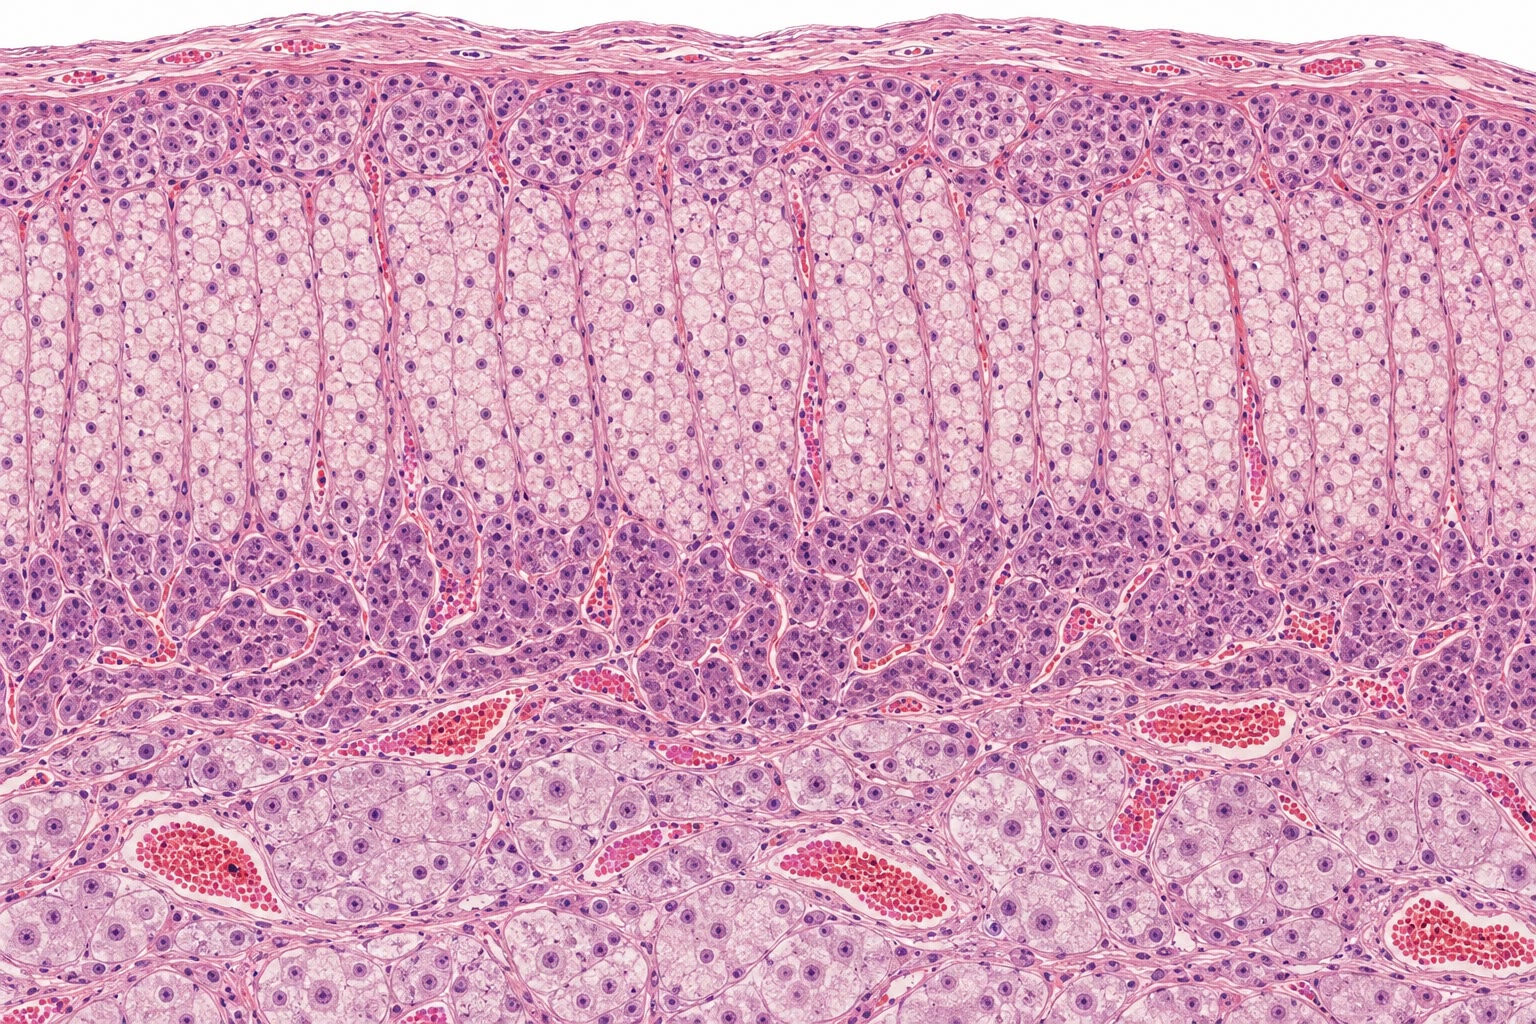
\includegraphics[width=0.5\linewidth]{images/book5/ai/b5-21-adrenal-section.jpg}\hspace{0.04\linewidth}
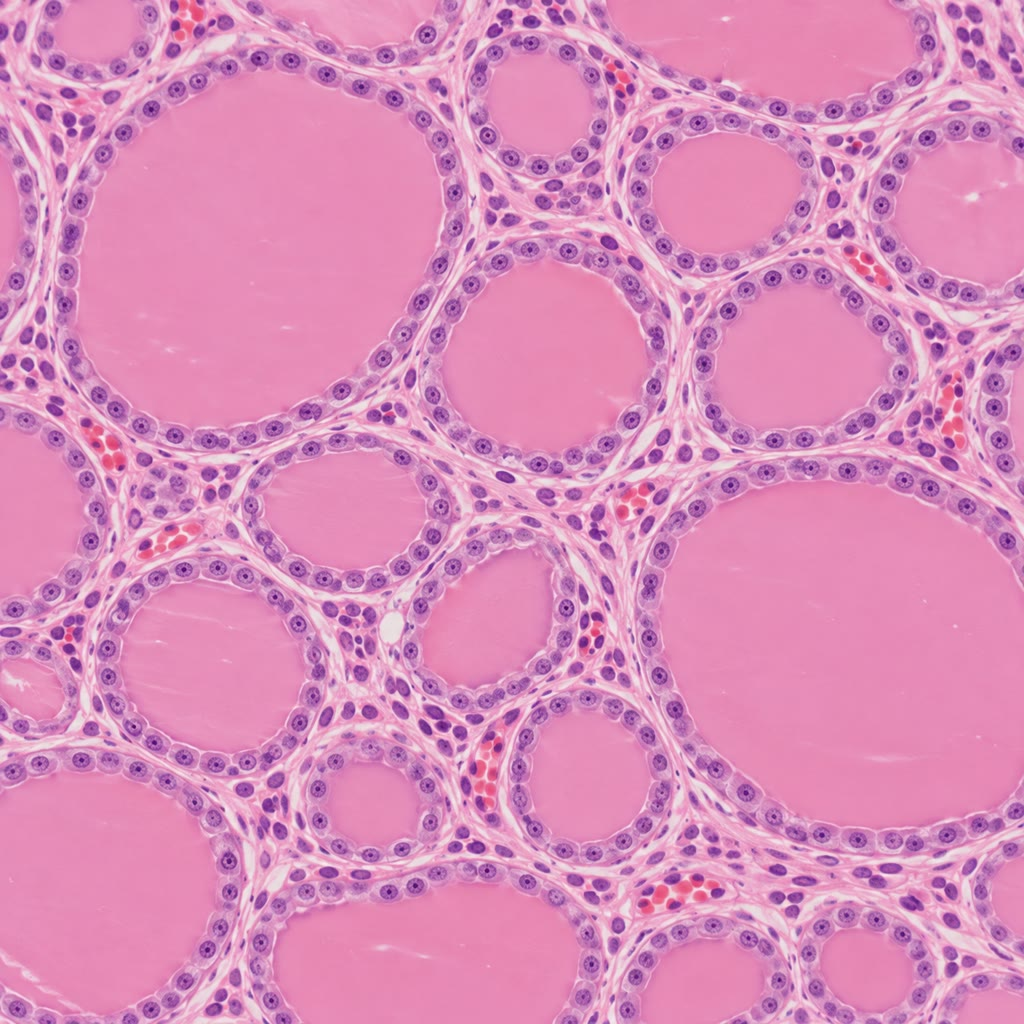
\includegraphics[width=0.36\linewidth]{images/book5/ai/b5-21-thyroid-follicles.jpg}

{\small बाएँ: काट में अधिवृक्क ग्रंथि --- अपने तीन क्षेत्रों में वल्कुट
(सबसे बाहर \omterm{def:b3:renal-osmoregulation:controls}{ऐल्डोस्टेरॉन}, चौड़े बीच के क्षेत्र में कॉर्टिसोल, सबसे भीतर
ऐंड्रोजन), और उसके भीतर एड्रिनैलीन-स्रावी क्रोमैफ़िन कोशिकाओं की कोई
मज्जा, जो उद्गम से कोई अनुकंपी \omterm{def:b3:nervous-systems:comparative}{गंडिका} है। दाएँ: अवटु पुटक, हर एक
कोशिकाओं का कोई गोला, जो कलिल के किसी ऐसे भंडार को घेरे है जिसमें
थायरोग्लोब्युलिन से बँधे महीनों भर के \omterm{def:b3:endocrinology:hormone}{हॉर्मोन} रखे हैं।}
\end{omfigure}

\section{ग्लूकोस: सबसे कसा हुआ पाश}

\begin{definition}[इंसुलिन और ग्लूकैगॉन]\label{def:b3:endocrinology:glucose}
\index{इंसुलिन}\index{ग्लूकैगॉन}\index{लैंगरहैंस की द्वीपिका}\index{GLUT4}\index{मधुमेह}
रक्त में लगभग \qty{5}{g} ग्लूकोस रहता है, \qty{5}{mmol/L} पर
(\qty{90}{mg/dL}), और मस्तिष्क दिन भर में \qty{120}{g} जलाता है तथा और
कुछ जला ही नहीं सकता; कोई भोजन घंटे भर में \qty{75}{g} पहुँचा देता है।
\emph{लैंगरहैंस की द्वीपिकाएँ}, यानी कुछ हज़ार कोशिकाओं के दस लाख
गुच्छे, जो अग्न्याशय भर बिखरे हैं, उस पाश को थामे हैं। $\beta$
कोशिकाएँ ग्लूकोस का उपापचय करके उसे भाँपती हैं: अधिक ग्लूकोस, अधिक ATP,
किसी ATP-संवेदी पोटैशियम वाहिका का बंद होना, विध्रुवण, कैल्सियम का
प्रवेश, और \emph{इंसुलिन} का बहिःकोशिकन, यानी किसी एक ही पूर्ववर्ती से
विदलित कोई \omterm{def:b3:endocrinology:hormone}{पेप्टाइड हॉर्मोन}। इंसुलिन पेशी तथा वसा से कहता है कि वाहक
\emph{GLUT4} अपने पृष्ठों पर ले आएँ और ग्लूकोस भीतर लें, यकृत से कि
ग्लूकोस ग्लाइकोजन के रूप में जमा करे और बनाना बंद करे, और वसा से कि
वसा अम्ल छोड़ना बंद करे: वह खाए हुए राज्य का \omterm{def:b3:endocrinology:hormone}{हॉर्मोन} है, और अकेला वही
रक्त-ग्लूकोस गिराता है। ग्लूकोस गिरने पर $\alpha$ कोशिकाएँ
\emph{ग्लूकैगॉन} छोड़ती हैं: यकृत ग्लाइकोजन तोड़ता है और ऐमीनो अम्लों
तथा लैक्टेट से नया ग्लूकोस बनाता है। एड्रिनैलीन, कॉर्टिसोल और वृद्धि
\omterm{def:b3:endocrinology:hormone}{हॉर्मोन} भी ग्लूकोस चढ़ाते हैं, और यह अनावश्यक-बहुलता सममित नहीं है:
कोई शरीर किसी गिरावट से चार रास्तों से बचाव कर सकता है और किसी बढ़त से
एक से। \emph{मधुमेह} उसी एक की विफलता है: प्ररूप 1, यानी $\beta$
कोशिकाओं का स्वप्रतिरक्षी विनाश, पहले ही दिन से इंसुलिन माँगता है;
प्ररूप 2, यानी दस में नौ मामले, ऊतकों के इंसुलिन-प्रतिरोध से शुरू होता
है, जिसे वर्षों तक और इंसुलिन से पूरा किया जाता है, जब तक $\beta$
कोशिकाएँ साथ न दे पाएँ और ग्लूकोस चढ़ जाए।
\end{definition}

\begin{theorem}[इंसुलिन--ग्लूकोस पाश]\label{thm:b3:endocrinology:loop}
\index{पाश-लाभ}\index{नियत बिंदु}\index{अवमंदित दोलन}
प्लाज़्मा ग्लूकोस और \omterm{def:b3:endocrinology:glucose}{इंसुलिन} के उनके उपवासी मानों से विचलनों के लिए
$g$ और $i$ लिखिए। ग्लूकोस अपनी ही अधिकता के समानुपाती दर से (यानी
ग्लूकोस-प्रभाविता $a$ से) और \omterm{def:b3:endocrinology:glucose}{इंसुलिन} की अधिकता के समानुपाती (संवेदनशीलता
$s$) साफ़ होता है; \omterm{def:b3:endocrinology:glucose}{इंसुलिन} ग्लूकोस की अधिकता के अनुपात में ($\beta$)
स्रवित होता है और दर $\gamma$ से साफ़; और कोई भार $u$ घुसता है:
\[
\dot g = -a\,g - s\,i + u, \qquad \dot i = \beta\,g - \gamma\,i .
\]
किसी स्थिर भार $u$ के तहत ग्लूकोस यहाँ जम जाता है
\[
g^{*} = \frac{u}{a}\cdot\frac{1}{1 + L}, \qquad L = \frac{s\beta}{a\gamma},
\]
इसलिए वह पुनर्भरण उस विक्षोभ को, जो किसी अनियंत्रित शरीर को झेलना
पड़ता, $1 + L$ से, यानी \emph{\omterm{thm:b3:endocrinology:loop}{पाश-लाभ}} जमा एक से, भाग देता है। किसी
बोलस के बाद वापसी अभिलक्षणिक मानों से शासित होती है,
$\lambda = -\tfrac{a + \gamma}{2} \pm \sqrt{\tfrac{(a+\gamma)^{2}}{4} - (a\gamma + s\beta)}$:
यदि $s\beta < (a - \gamma)^{2}/4$ हो तो एकदिष्ट, और अन्यथा कोणीय
आवृत्ति $\omega = \sqrt{a\gamma + s\beta -
(a+\gamma)^{2}/4}$ का कोई \omterm{thm:b3:endocrinology:loop}{अवमंदित दोलन}, जो $\mathrm{e}^{-(a+\gamma)t/2}$
की तरह क्षीण होता है --- यानी ग्लूकोस जमने से पहले अपने उपवासी मान से
नीचे उतर जाता है, और वही किसी मीठे भोजन के दो-तीन घंटे बाद की हलकी
अल्पग्लूकोजता है। इंसुलिन-प्रतिरोध $s$ गिरा देता है: शरीर के अपने
यकृतीय निर्गम के तहत उपवासी स्थायी अवस्था चढ़ जाती है, और वह पाश किसी
ऊँचे $i^{*}$ से भरपाई करता रहता है, जब तक $\beta$ कोशिकाओं का $\beta$
भी न गिरे, और तब वह भरपाई विफल हो जाती है।
\end{theorem}
\begin{proof}
स्थायी अवस्था: $\dot i = 0$ से $i^{*} = \beta g^{*}/\gamma$ मिलता है;
उसे $\dot g = 0$ में रखने पर: $a g^{*} + s\beta g^{*}/\gamma = u$,
जिससे $g^{*} =
u/(a + s\beta/\gamma) = (u/a)/(1 + L)$। गतिकी: निकाय-आव्यूह
$\begin{pmatrix} -a & -s\\ \beta & -\gamma\end{pmatrix}$ है, जिसका
अनुरेख $-(a+\gamma)$ है और सारणिक $a\gamma + s\beta$; और उसके
अभिलक्षणिक समीकरण $\lambda^{2} + (a+\gamma)\lambda + (a\gamma + s\beta) = 0$
के मूल वही हैं जो बताए गए। दोनों का वास्तविक भाग ऋणात्मक है, इसलिए वह
उपवासी अवस्था स्थिर है; वे मूल तब सम्मिश्र होते हैं जब विविक्तकर
$(a+\gamma)^{2}
- 4(a\gamma + s\beta) = (a-\gamma)^{2} - 4s\beta$ ऋणात्मक हो, यानी वही
दी गई शर्त, और तब $g(t) = \mathrm{e}^{-(a+\gamma)t/2}(A\cos\omega t
+ B\sin\omega t)$, जो शून्य पार करता है। प्रतिरोध: $u$ को यकृत का
आधारी निर्गम और $s$ को घटा हुआ लेने पर, $L$ गिरता है और $g^{*}$ उसी
$u$ के लिए चढ़ता है; $i^{*} = \beta g^{*}/\gamma$ उसके साथ चढ़ता है
(अतिइंसुलिनता); और यदि फिर $\beta$ गिरे, तो $L$ और गिरता है तथा
$g^{*}$ $u/a$ की ओर चढ़ता जाता है।
\end{proof}

\begin{omfigure}
\begin{tikzpicture}
\begin{axis}[
  width=0.58\linewidth, height=5.6cm,
  axis x line=bottom, axis y line=left,
  xmin=0, xmax=180, ymin=40, ymax=200,
  xlabel={ग्लूकोस बोलस के बाद के मिनट}, ylabel={प्लाज़्मा ग्लूकोस (mg/dL)},
  xlabel style={font=\small, at={(axis description cs:0.5,-0.12)}, anchor=north}, ylabel style={font=\small},
  tick label style={font=\small}, xtick={0,30,60,90,120,150,180}, ytick={60,90,120,150,180},
  clip=false,
]
\addplot[very thick, omDef, smooth] coordinates {(0,190) (6,165) (12,131) (18,102) (24,84) (30,77) (36,78) (42,82) (48,86) (54,89) (60,91) (66,92) (72,91) (78,91) (84,90) (90,90) (96,90) (102,90) (108,90) (114,90) (120,90) (126,90) (132,90) (138,90) (144,90) (150,90) (156,90) (162,90) (168,90) (174,90) (180,90)};
\draw[dashed, gray] (axis cs:0,90) -- (axis cs:180,90);
\node[font=\scriptsize, gray, anchor=south east] at (axis cs:180,91) {उपवासी स्तर};
\node[font=\scriptsize, omDef, anchor=west, align=left] at (axis cs:75,150) {प्रतिरूप: $a = \qty{0.02}{min^{-1}}$, $\gamma = \qty{0.1}{min^{-1}}$,\\$s\beta = \qty{0.01}{min^{-2}}$, पाश-लाभ $L = 5$;\\\qty{32}{min} पर अधोउछाल, आवर्तकाल \qty{68}{min}};
\node[font=\scriptsize, omThm, anchor=north] at (axis cs:24,70) {अधोउछाल};
\end{axis}
\begin{axis}[
  at={(0.6\linewidth,0)}, anchor=south west,
  width=0.33\linewidth, height=5.6cm,
  axis x line=bottom, axis y line=left,
  xmin=0, xmax=180, ymin=0, ymax=40,
  xlabel={मिनट}, ylabel={इंसुलिन (mU/L)},
  xlabel style={font=\small, at={(axis description cs:0.5,-0.12)}, anchor=north}, ylabel style={font=\small},
  tick label style={font=\small}, xtick={0,60,120,180}, ytick={0,10,20,30,40},
]
\addplot[very thick, omProp, smooth] coordinates {(0,10.0) (6,30.0) (12,33.7) (18,28.5) (24,20.4) (30,13.4) (36,8.9) (42,7.1) (48,7.1) (54,7.9) (60,9.0) (66,9.8) (72,10.2) (78,10.4) (84,10.4) (90,10.2) (96,10.1) (102,10.0) (108,10.0) (114,9.9) (120,10.0) (126,10.0) (132,10.0) (138,10.0) (144,10.0) (150,10.0) (156,10.0) (162,10.0) (168,10.0) (174,10.0) (180,10.0)};
\draw[dashed, gray] (axis cs:0,10) -- (axis cs:180,10);
\end{axis}
\end{tikzpicture}

{\small किसी ऐसे बोलस के बाद वह रैखिक पाश, जो ग्लूकोस को
\qty{100}{mg/dL} चढ़ा देता है। \omterm{def:b3:endocrinology:glucose}{इंसुलिन} दस मिनटों के भीतर शिखर छूता है
और ग्लूकोस बीस में आधार पर लौट आता है, फिर नीचे उतर जाता है; कोई प्रबल
पुनर्भरण, जो किसी ऐसे \omterm{def:b3:endocrinology:hormone}{हॉर्मोन} के ज़रिए काम करे जिसका अपना सफ़ाई-काल हो,
किसी सादे क्षय के बजाय किसी \omterm{thm:b3:endocrinology:loop}{अवमंदित दोलन} के रूप में लौटता है।}
\end{omfigure}

\begin{proof}[प्रमाण-सामग्री]
फ़ोन मेरिंग और मिंकोव्स्की (1889) ने किसी कुत्ते का अग्न्याशय निकालकर
\omterm{def:b3:endocrinology:glucose}{मधुमेह} पैदा कर दिया --- उसके मूत्र पर जुटती मक्खियों ने वह शर्करा खोल
दी; और नलिकाएँ बाँधने से, जिससे पाचक ऊतक नष्ट हुआ पर द्वीपिकाएँ बच
गईं, ऐसा नहीं हुआ। बैंटिंग और बेस्ट (1921) ने, कॉलिप के शोधन के साथ, वह
द्वीपिका-तत्त्व निकाला और किसी मधुमेही कुत्ते का रक्त-शर्करा गिराया,
और फिर लियोनार्ड थॉम्प्सन का (जनवरी 1922)। सैंगर ने \omterm{def:b3:endocrinology:glucose}{इंसुलिन} अनुक्रमित
किया (1955), यानी पहला प्रोटीन अनुक्रम; यालो और बर्सन ने उसे रक्त में
नापा (1959) और पाया कि वयस्क-आरंभ मधुमेहियों में वह, कम से कम पहले,
स्वस्थ लोगों से अधिक था --- यानी प्रतिरोध, न्यूनता नहीं। जेनेनटेक के
जीवाणुओं ने 1978 में मानव \omterm{def:b3:endocrinology:glucose}{इंसुलिन} बनाया, यानी पहली पुनर्योगज औषध।
\end{proof}

\begin{omfigure}
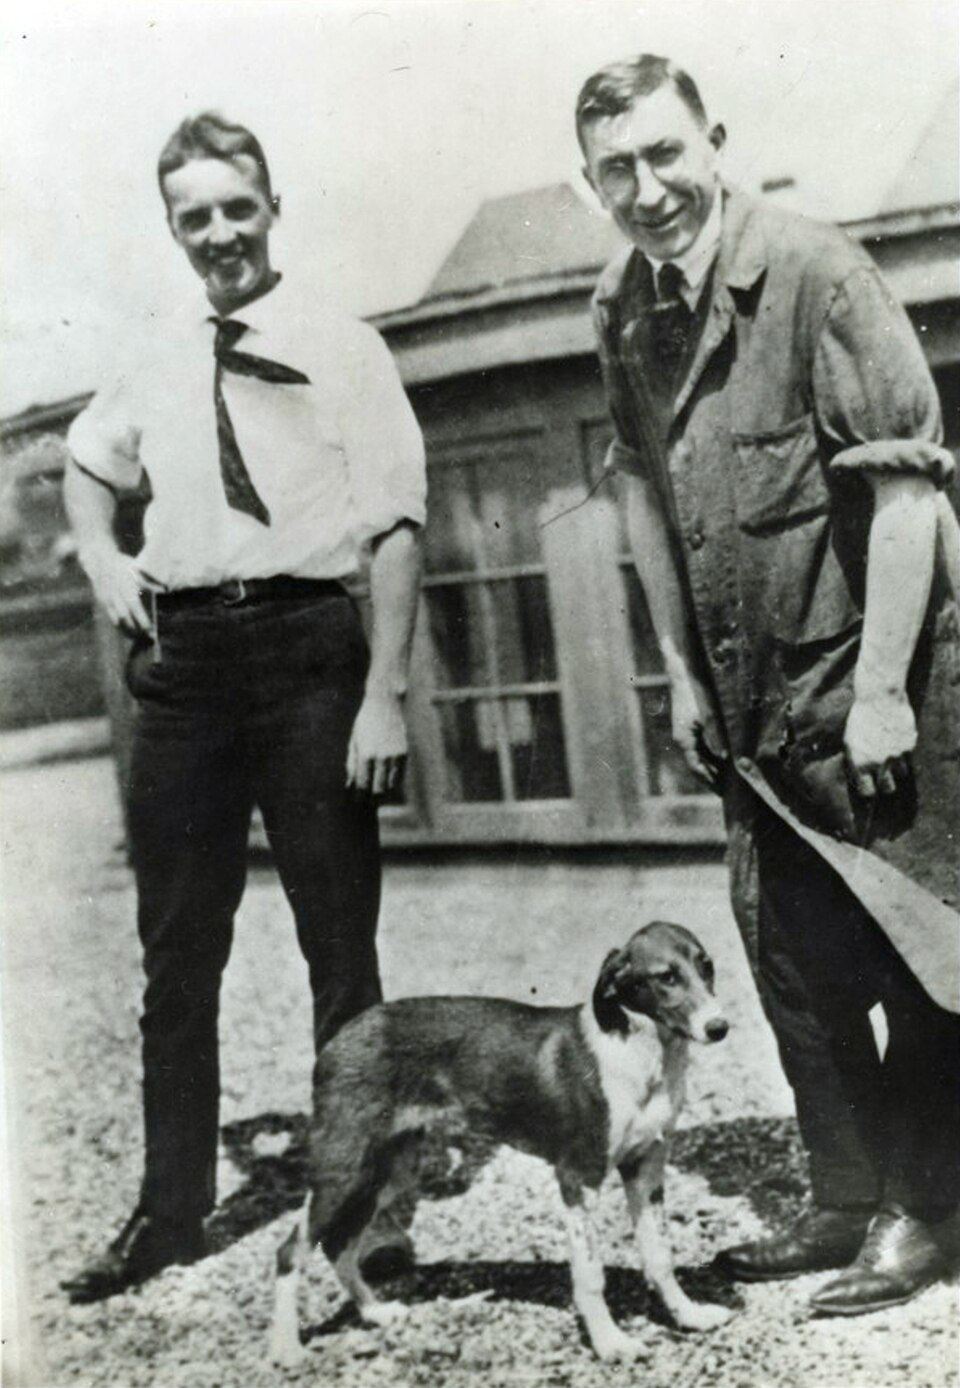
\includegraphics[width=0.42\linewidth]{images/book5/banting-best.jpg}\hspace{0.04\linewidth}
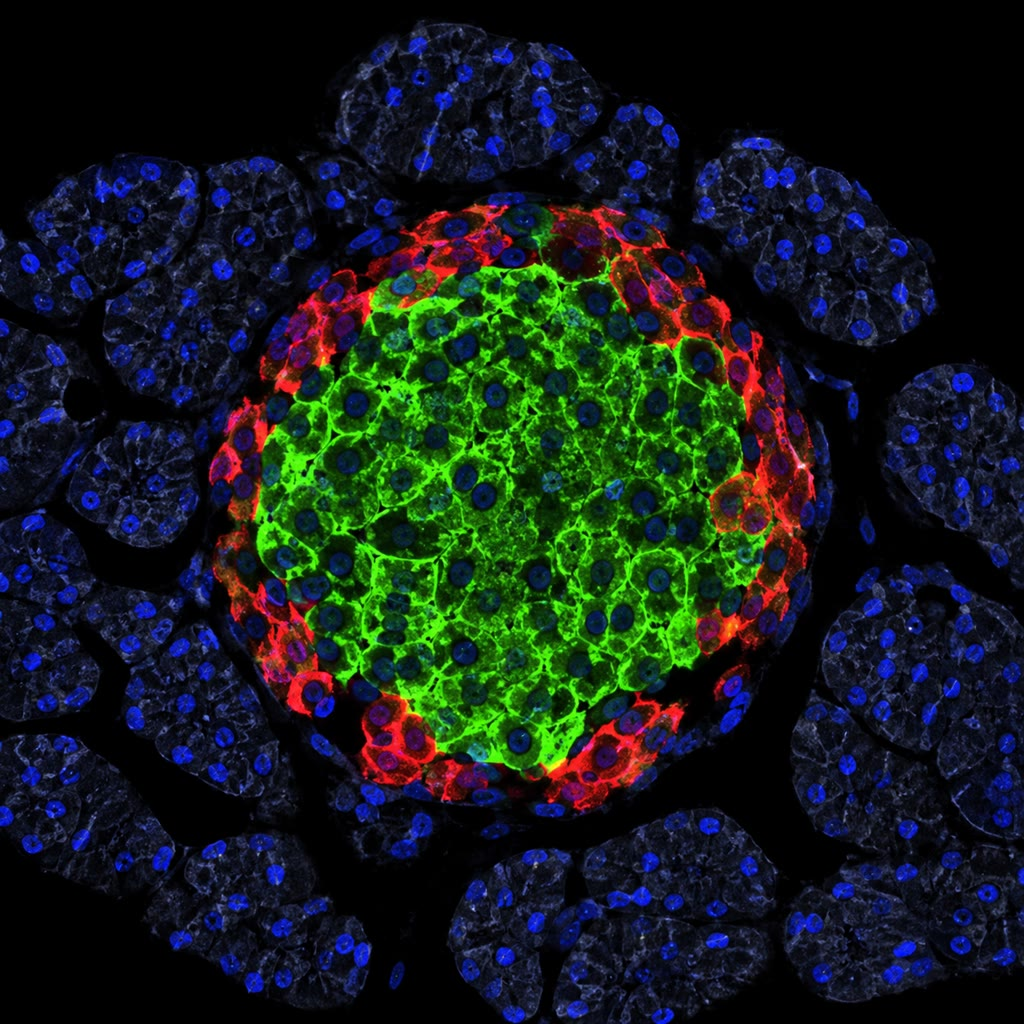
\includegraphics[width=0.42\linewidth]{images/book5/ai/b5-21-pancreatic-islet.jpg}

{\small बाएँ: फ़्रेडरिक बैंटिंग और चार्ल्स बेस्ट, लगभग 1924 में, टोरंटो
की चिकित्सा इमारत की छत पर, इंसुलिन-प्रयोगों के किसी कुत्ते के साथ
(सार्वजनिक छायाचित्र)। दाएँ: लैंगरहैंस की कोई द्वीपिका, केंद्र में
\omterm{def:b3:endocrinology:glucose}{इंसुलिन} बनाती $\beta$ कोशिकाएँ, किनारे पर \omterm{def:b3:endocrinology:glucose}{ग्लूकैगॉन} वाली $\alpha$
कोशिकाएँ, बहिःस्रावी कोष्ठकों के किसी समुद्र में।}
\end{omfigure}

\begin{method}[किसी रोगी में ग्लूकोस-पाश पढ़ना]\label{met:b3:endocrinology:ogtt}
\index{ग्लूकोस सह्यता परीक्षण}\index{HbA1c}
(1) उपवासी प्लाज़्मा ग्लूकोस: सामान्य \qty{5.6}{mmol/L} से नीचे,
\omterm{def:b3:endocrinology:glucose}{मधुमेह} दो मौकों पर \qty{7.0}{mmol/L} पर या उससे ऊपर। (2) मौखिक \omterm{met:b3:endocrinology:ogtt}{ग्लूकोस
सह्यता परीक्षण}: \qty{75}{g} ग्लूकोस पिलाया जाता है; दो घंटे पर
प्लाज़्मा ग्लूकोस सामान्य \qty{7.8}{mmol/L} से नीचे, \omterm{def:b3:endocrinology:glucose}{मधुमेह}
\qty{11.1}{mmol/L} पर या उससे ऊपर --- दो घंटे वाला मान उस पाश का लाभ
पढ़ता है, और उपवासी मान उसका \omterm{thm:b3:endocrinology:loop}{नियत बिंदु}। (3) ग्लाइकेटित हीमोग्लोबिन,
यानी \emph{HbA1c}: ग्लूकोस अपनी सांद्रता के समानुपाती दर से
हीमोग्लोबिन से अनुत्क्रमणीय रूप से चिपकता है, और लोहिताणु 120 दिन जीते
हैं, इसलिए ग्लाइकेटित अंश बिना किसी उपवास के पिछले तीन महीनों का माध्य
ग्लूकोस समाकलित कर देता है --- सामान्य \qty{5.7}{\%} से नीचे, \omterm{def:b3:endocrinology:glucose}{मधुमेह}
\qty{6.5}{\%} से। (4) प्रतिरोध को न्यूनता से अलग करने के लिए, साथ में
\omterm{def:b3:endocrinology:glucose}{इंसुलिन} (या उसका उपोत्पाद C-पेप्टाइड) नापिए: ऊँचे ग्लूकोस के साथ ऊँचा
\omterm{def:b3:endocrinology:glucose}{इंसुलिन} प्रतिरोध है; और अनुपस्थित C-पेप्टाइड प्ररूप~1।
\end{method}

\section{कैल्सियम, और वह घड़ी}

\begin{definition}[कैल्सियम का समस्थापन]\label{def:b3:endocrinology:calcium}
\index{परावटु हॉर्मोन}\index{कैल्सिट्रिऑल}\index{विटामिन D}\index{अस्थिसुषिरता}
प्लाज़्मा का आयनित कैल्सियम \qty{1.2}{mmol/L} पर कुछ ही प्रतिशत के
भीतर थमा रहता है, क्योंकि वही हर तंत्रिका तथा पेशी की उत्तेजनीयता तय
करता है: बहुत कम हो तो वे अपने आप दगने लगती हैं (टेटनी), बहुत अधिक हो
तो वे सुस्त पड़ जाती हैं। चारों परावटु ग्रंथियाँ उसे किसी पृष्ठीय
ग्राही से भाँपती हैं और \emph{परावटु \omterm{def:b3:endocrinology:hormone}{हॉर्मोन}} (PTH) किसी तीखे व्युत्क्रम
सिग्मॉइड के अनुदिश स्रवित करती हैं: PTH अस्थि से कैल्सियम लामबंद करता
है, गुर्दे से उसे पुनःसोखवाता तथा फ़ॉस्फ़ेट उत्सर्जित करवाता है, और
\emph{विटामिन D} सक्रिय करता है --- जो त्वचा में पराबैंगनी प्रकाश से
बनता है या खाया जाता है, यकृत में और फिर गुर्दे में हाइड्रॉक्सिलित होकर
\emph{कैल्सिट्रिऑल} बनता है --- जो आँत से कैल्सियम अवशोषित करवाता है।
अस्थि वह भंडार है, यानी किलोग्राम भर कैल्सियम, जिसका पुनर्निर्माण
अस्थिभंजक तथा अस्थिकोरक PTH, कैल्सिट्रिऑल, एस्ट्रोजन और भार के तहत
लगातार करते रहते हैं। विटामिन D की कमी बच्चों में सूखा रोग और वयस्कों
में नरम हड्डियाँ देती है; रजोनिवृत्ति पर एस्ट्रोजन का गिरना उस
पुनर्निर्माण को अवशोषण की ओर झुका देता है और \emph{अस्थिसुषिरता} देता
है; और कोई परावटु \omterm{def:b3:cancer-biology:hallmarks}{अर्बुद} कैल्सियम चढ़ा देता है, अस्थि घोल देता है और
गुर्दे में पथरी बना देता है --- ``हड्डियाँ, पथरियाँ, कराहें और
कलपनाएँ।''
\end{definition}

\begin{definition}[दैनिक घड़ी]\label{def:b3:endocrinology:clock}
\index{दैनिक घड़ी}\index{अधिदृक्-संधि गुठली}\index{घड़ी जीन}\index{मेलाटोनिन}\index{कालदाता}
लगभग हर कोशिका कोई \emph{दैनिक घड़ी} ढोती है: कोई
अनुलेखन--अनुवादन पाश, जिसमें प्रोटीन CLOCK और BMAL1 जीन \emph{Per}
तथा \emph{Cry} चालू कर देते हैं, जिनके प्रोटीन जमा होते हैं, घंटों के
किसी विलंब के बाद केंद्रक में घुसते हैं और अपना ही अनुलेखन दबा देते
हैं, फिर अपघटित हो जाते हैं, जिससे वह दमन हट जाता है --- यानी लगभग
चौबीस घंटों में एक चक्र, जो उस विलंब और उस अपघटन की दरों से तय होता है।
शरीर की घड़ियाँ \omterm{def:b3:endocrinology:axes}{अधश्चेतक} की \emph{अधिदृक्-संधि गुठली} के बीस हज़ार
न्यूरॉनों की किसी स्वामी घड़ी से समकालिक होती हैं, जो स्वयं \omterm{def:b3:sensory-systems:retina}{दृष्टिपटल}
की \omterm{def:b3:sensory-systems:retina}{गंडिका कोशिकाओं} के किसी समर्पित वर्ग के ज़रिए (जिसमें मेलेनॉप्सिन
है, \omterm{def:b3:sensory-systems:retina}{शलाकाओं} या \omterm{def:b3:sensory-systems:retina}{शंकुओं} के वर्णक नहीं) प्रकाश से सेट होती है, और जो
पीनियल के \emph{मेलाटोनिन} के ज़रिए शरीर को रात का संकेत देती है, जो
केवल अँधेरे में स्रवित होता है। वह घड़ी जागने से पहले कॉर्टिसोल तय करती
है, देह-तापमान सुबह 4 बजे सबसे नीचा, पहली नींद में वृद्धि \omterm{def:b3:endocrinology:hormone}{हॉर्मोन}, और
सुबह इंसुलिन-संवेदनशीलता ऊँची; और भोजन, व्यायाम तथा तापमान गौण
\emph{कालदाता} हैं, जो परिधीय घड़ियों को केंद्रीय से दूर खींच सकते हैं,
और वही पाली-कर्मी की तथा कालक्षेत्र-श्रांति की बेचैनी है --- यानी एक
समय पर चलती यकृत की घड़ी और दूसरे पर मस्तिष्क की।
\end{definition}

\begin{proof}[प्रमाण-सामग्री]
कोनोपका और बेंज़र (1971) ने उत्परिवर्ती मक्खियों को उनके निकलने की बदली
हुई लयों के लिए छाना और किसी एक जीन, \emph{period}, के तीन युग्मविकल्पी
पाए: कोई छोटा दिन (19 घं.), कोई लंबा दिन (29 घं.), और कोई लय ही नहीं
--- यानी कोई ऐसी घड़ी जिसका आवर्तकाल आनुवंशिक है। हार्डिन, हॉल और
रॉसबैश (1990) ने पाया कि \emph{period} का mRNA तथा प्रोटीन अपने बीच के
किसी अंतराल के साथ दोलन करते हैं, और कि वह प्रोटीन अपने ही जीन को दबाता
है: यानी वह पाश। रैल्फ़ और मेनेकर (1990) ने 20 घंटे की लय वाले किसी
उत्परिवर्ती हैम्स्टर की \omterm{def:b3:endocrinology:clock}{अधिदृक्-संधि गुठली} किसी ऐसे सामान्य हैम्स्टर
में प्रत्यारोपित की जिसकी अपनी गुठली नष्ट कर दी गई थी: वह ग्रहीता 20
घंटों पर चला --- यानी वह आवर्तकाल उसी प्रत्यारोपित ऊतक का था। बिना
काल-संकेतों के किसी तहख़ाने में रखे मनुष्यों में वह लय 24 घंटे से
थोड़ा ऊपर मुक्त चली; शाम की कोई तेज़ रोशनी उसे पीछे खिसकाती थी और सुबह
की आगे।
\end{proof}

\begin{omfigure}
\begin{tikzpicture}[every node/.style={font=\scriptsize}, >=stealth]
  \node[draw, thick, rounded corners, fill=omDef!20, align=center] (cb) at (0,1.6) {CLOCK--BMAL1\\सक्रियक};
  \node[draw, thick, rounded corners, fill=omProp!25, align=center] (pc) at (3.6,1.6) {\emph{Per}, \emph{Cry}\\अनुलेखित};
  \node[draw, thick, rounded corners, fill=omThm!20, align=center] (pr) at (3.6,-0.4) {PER, CRY प्रोटीन\\जमा होते, द्विलक बनते};
  \node[draw, thick, rounded corners, fill=omMeth!25, align=center] (nu) at (0,-0.4) {घंटों बाद\\केंद्रक में घुसते};
  \draw[->, thick] (cb) -- (pc) node[midway, above, font=\tiny] {सक्रिय करते};
  \draw[->, thick] (pc) -- (pr) node[midway, right, font=\tiny] {अनुवादन, विलंब};
  \draw[->, thick] (pr) -- (nu);
  \draw[-|, thick, omThm] (nu) -- (cb) node[midway, left, font=\tiny, omThm, align=right] {अपने ही\\सक्रियक\\दबाते};
  \draw[->, thick, gray] (nu.south) -- ++(0,-0.5) node[below, font=\tiny, gray] {अपघटित: दमन हटता है, चक्र फिर शुरू $\approx$ \qty{24}{h}};
  % right: daily profile
  \begin{scope}[shift={(7.2,-1.6)}]
    \draw[->] (0,0) -- (5.6,0) node[right, font=\tiny] {घंटा};
    \draw[->] (0,0) -- (0,3.4);
    \foreach \x/\l in {0/0, 1.4/6, 2.8/12, 4.2/18, 5.6/24} { \draw (\x,0) -- (\x,-0.08) node[below, font=\tiny] {\l}; }
    \fill[gray!25] (0,0) rectangle (1.4,3.4); \fill[gray!25] (5.1,0) rectangle (5.6,3.4);
    \node[font=\tiny, gray!60!black] at (0.7,3.2) {रात};
    \draw[very thick, omMeth!70!black, domain=0:5.6, samples=60, smooth, variable=\x] plot (\x, {1.6 + 1.2*cos(deg(2*3.1416*(\x-1.9)/5.6))});
    \node[font=\tiny, omMeth!70!black] at (3.1,3.1) {कॉर्टिसोल: शिखर सुबह 8 बजे};
    \draw[very thick, omDef, domain=0:5.6, samples=60, smooth, variable=\x] plot (\x, {0.9 + 0.7*cos(deg(2*3.1416*(\x-0.7)/5.6))});
    \node[font=\tiny, omDef] at (2.7,0.18) {मेलाटोनिन: केवल रात};
  \end{scope}
\end{tikzpicture}

{\small बाएँ: उस आणविक घड़ी का केंद्र, यानी घंटों के विलंब वाला कोई
\omterm{def:b3:endocrinology:axes}{ऋणात्मक पुनर्भरण} पाश, जो किसी पाश को जमने के बजाय दोलन करने के लिए
चाहिए। दाएँ: उसके तय किए दो \omterm{def:b3:endocrinology:hormone}{हॉर्मोन} --- दिन की तैयारी के लिए भोर से
पहले चढ़ता कॉर्टिसोल, और रात को चिह्नित करता \omterm{def:b3:endocrinology:clock}{मेलाटोनिन}।}
\end{omfigure}

\begin{remark}[नियंत्रण के रूप में समस्थापन]\label{rem:b3:endocrinology:control}
इस अध्याय के हर पाश के वही पुर्ज़े हैं: कोई संवेदक ($\beta$ कोशिका का
उपापचय, परावटु का कैल्सियम-ग्राही, \omterm{def:b3:endocrinology:axes}{पीयूष} का अवटु-हॉर्मोन ग्राही), कोई
नियंत्रक जो किसी \omterm{thm:b3:endocrinology:loop}{नियत बिंदु} से तुलना करे, कोई कारक \omterm{def:b3:endocrinology:hormone}{हॉर्मोन} जिसका अपना
अर्ध-आयु काल हो, और कोई पुनर्भरण जो उस त्रुटि को $1 + L$ के गुणक से
घटाए पर कभी शून्य तक नहीं। जो भिन्न है वह समय है --- एड्रिनैलीन के लिए
सेकंड, \omterm{def:b3:endocrinology:glucose}{इंसुलिन} के लिए घंटा, थायरॉक्सिन के लिए दिन, अस्थि के लिए जीवन भर
--- और उस समझौते की कीमत: विलंबित कारक वाला कोई तेज़ पाश दोलन करता है,
और कोई धीमा पाश किसी विक्षोभ को टिकने देता है। चिकित्सालय उन पाशों को
बाहर से देखता है, उन जोड़ों के ज़रिए जिन्हें वह पुनर्भरण युग्मित करता
है: कम T$_{4}$ के साथ ऊँचा TSH कोई विफल ग्रंथि है, और ऊँचे T$_{4}$ के
साथ ऊँचा TSH कोई विफल \omterm{def:b3:endocrinology:axes}{पीयूष}; ऊँचे ग्लूकोस के साथ ऊँचा \omterm{def:b3:endocrinology:glucose}{इंसुलिन} प्रतिरोध
है, और ऊँचे ग्लूकोस के साथ कम \omterm{def:b3:endocrinology:glucose}{इंसुलिन} विनाश। किसी \omterm{def:b3:endocrinology:hormone}{हॉर्मोन} का स्तर
पढ़ने के लिए यह पूछना ही पड़ता है कि उसका सेनापति क्या कर रहा था।
\end{remark}

\section{अभ्यास}

\begin{exercise}[$\star$]\label{exo:b3:endocrinology:1}
\omterm{def:b3:endocrinology:glucose}{इंसुलिन}, कॉर्टिसोल, एड्रिनैलीन, थायरॉक्सिन और वैसोप्रेसिन को रसायन,
ग्राही की जगह, क्रिया की गति और अर्ध-आयु काल से वर्गीकृत कीजिए।
\end{exercise}

\begin{exercise}[$\star$]\label{exo:b3:endocrinology:2}
अवटु अक्ष उसके पुनर्भरण के साथ खींचिए और इनमें TSH तथा T$_{4}$ का
पूर्वानुमान कीजिए: कोई नष्ट अवटु; TSH स्रवित करता कोई \omterm{def:b3:endocrinology:axes}{पीयूष} \omterm{def:b3:cancer-biology:hallmarks}{अर्बुद};
बहुत अधिक थायरॉक्सिन लेता कोई रोगी; आयोडीन की कमी।
\end{exercise}

\begin{exercise}[$\star$]\label{exo:b3:endocrinology:3}
किसी शरीर के पास रक्त-ग्लूकोस चढ़ाने वाले चार \omterm{def:b3:endocrinology:hormone}{हॉर्मोन} और गिराने वाला
केवल एक क्यों है? इससे बहुत अधिक और बहुत कम \omterm{def:b3:endocrinology:glucose}{इंसुलिन} के सापेक्ष ख़तरों
के बारे में क्या पूर्वानुमान निकलता है?
\end{exercise}

\begin{exercise}[$\star$]\label{exo:b3:endocrinology:4}
\omterm{def:b3:endocrinology:clock}{कालदाता} क्या है? तीन दीजिए, बताइए कि स्वामी घड़ी कौन-सा काम में लेती
है, और समझाइए कि आठ कालक्षेत्र पार करते किसी यात्री का क्या होता है।
\end{exercise}

\begin{exercise}[$\star\star$]\label{exo:b3:endocrinology:5}
किसी कोशिका के \num{20000} ग्राही हैं जिनका $K_{d} = \qty{1}{nM}$ है और
वह तब अधिकतम अनुक्रिया देती है जब \num{500} अधिकृत हों। EC$_{50}$
खोजिए। ऊँचे \omterm{def:b3:endocrinology:hormone}{हॉर्मोन} के हफ़्ते भर बाद उस कोशिका के \num{2000} ग्राही
हैं: नया EC$_{50}$? इंसुलिन-प्रतिरोध के लिए इसकी व्याख्या कीजिए।
\end{exercise}

\begin{exercise}[$\star\star$]\label{exo:b3:endocrinology:6}
$\kappa = \qty{0.46}{L/pmol}$ के साथ और मुक्त T$_{4}$ के
\qty{15}{pmol/L} पर सामान्य TSH \qty{1.5}{mU/L} के साथ, T$_{4}$ के
$13$, $11$, $9$ और \qty{25}{pmol/L} होने पर TSH निकालिए। इनमें से किस
पर T$_{4}$ \qtyrange{10}{20}{pmol/L} की संदर्भ परास के भीतर होता जबकि
TSH \qtyrange{0.4}{4}{mU/L} के बाहर?
\end{exercise}

\begin{exercise}[$\star\star$]\label{exo:b3:endocrinology:7}
\cref{thm:b3:endocrinology:loop} के पाश में, $a = \qty{0.02}{min^{-1}}$,
$\gamma = \qty{0.1}{min^{-1}}$, प्रति mg/dL
$\beta = \qty{0.05}{mU\,L^{-1}\,min^{-1}}$
और प्रति mU/L $s = \qty{0.2}{mg\,dL^{-1}\,min^{-1}}$ के साथ, \omterm{thm:b3:endocrinology:loop}{पाश-लाभ},
\qty{2}{mg/dL/min} के किसी अचर भार के तहत स्थायी ग्लूकोस-अधिकता, वही
बिना पुनर्भरण के, और स्थायी इंसुलिन-अधिकता निकालिए।
\end{exercise}

\begin{exercise}[$\star\star$]\label{exo:b3:endocrinology:8}
वही प्राचल: किसी बोलस के बाद वापसी दोलनी है? आवर्तकाल और आयाम के
$\mathrm{e}$ गुना गिरने का समय निकालिए। अब $s$ आधा कीजिए
(इंसुलिन-प्रतिरोध): दोनों और नया \omterm{thm:b3:endocrinology:loop}{पाश-लाभ} फिर से निकालिए।
\end{exercise}

\begin{exercise}[$\star\star$]\label{exo:b3:endocrinology:9}
कॉर्टिसोल का अर्ध-आयु काल \qty{80}{min} है। साल भर रोज़
\qty{40}{mg} प्रेडनिसोलोन पर रहा कोई रोगी उसे अचानक बंद कर देता है।
तह-दर-तह समझाइए कि वह तीन दिन बाद किसी मामूली संक्रमण में क्यों ढह
सकता है, और वह अक्ष नापा जाए तो क्या दिखाता (ACTH, कॉर्टिसोल,
अंतःक्षिप्त ACTH पर अनुक्रिया)।
\end{exercise}

\begin{exercise}[$\star\star\star$]\label{exo:b3:endocrinology:10}
दिखाइए कि कोई एक-चर \omterm{def:b3:endocrinology:axes}{ऋणात्मक पुनर्भरण} $\dot x = f(x)$, जिसमें
$f' < 0$ हो, दोलन नहीं कर सकता, जबकि प्रमेय का दो-चर पाश कर सकता है, और शब्दों में
समझाइए कि 24 घंटे का आवर्तकाल बनाने के लिए उस घड़ी को अनुलेखन और दमन के
बीच घंटों का विलंब क्यों चाहिए। यदि PER दुगुनी तेज़ी से अपघटित हो तो
उस आवर्तकाल का क्या होगा?
\end{exercise}

\begin{exercise}[$\star\star\star$]\label{exo:b3:endocrinology:11}
\omterm{def:b3:endocrinology:calcium}{परावटु हॉर्मोन} $\text{PTH} = P_{\max}/(1 +
\mathrm{e}^{k(\text{Ca} - \text{Ca}_{0})})$ मानता है, जिसमें $\text{Ca}_{0} =
\qty{1.2}{mmol/L}$ और $k = \qty{20}{L/mmol}$ है। Ca
$= 1.10$, $1.15$, $1.20$, $1.25$ और \qty{1.30}{mmol/L} पर PTH को अधिकतम
के अंश के रूप में निकालिए, \omterm{thm:b3:endocrinology:loop}{नियत बिंदु} पर ढाल निकालिए, और समझाइए कि ऐसी
तीखी ढाल कैल्सियम के लिए क्यों चाही जाती है पर ग्लूकोस के लिए
ख़तरनाक होती।
\end{exercise}

\begin{exercise}[$\star\star\star$]\label{exo:b3:endocrinology:12}
ग्लूकोस हीमोग्लोबिन से प्रति एकांक समय दर $k\,G$ से चिपकता है, जिसमें
$k$ ऐसा है कि \qty{5.5}{mmol/L} का कोई माध्य ग्लूकोस किसी लोहिताणु के
120 दिन के जीवन भर में \qty{5}{\%} ग्लाइकेशन देता है। HbA1c को माध्य
ग्लूकोस के किसी फलन के रूप में व्युत्पन्न कीजिए, \qty{10}{mmol/L} पर
उसका मान, और समझाइए कि रक्तलयी अरक्तता वाले किसी रोगी (जिसके लोहिताणु
60 दिन जीते हैं) का HbA1c भ्रामक रूप से कम क्यों होता है।
\end{exercise}

\section{समस्या: रक्त की शर्करा}

\begin{problem}[{सप्तांत समस्या --- रैखिक इंसुलिन--ग्लूकोस पाश से पढ़ा
गया कोई \omterm{met:b3:endocrinology:ogtt}{ग्लूकोस सह्यता परीक्षण}: \qty{75}{g} मात्रा का वितरण, \omterm{thm:b3:endocrinology:loop}{पाश-लाभ}
और अवमंदित वापसी, प्रतिरोध तथा $\beta$-कोशिका विफलता उपवासी \omterm{thm:b3:endocrinology:loop}{नियत बिंदु}
का क्या करते हैं, संख्याओं से कोई निदान, और उसके बगल में अवटु अक्ष,
जिसका अंत \omterm{thm:b3:endocrinology:loop}{पाश-लाभ} पर होता है, वापसी के समय पर, और विफल होते पाश के
उपवासी ग्लूकोस पर}]
\label{pb:b3:endocrinology:1}
आँकड़े: कोई स्वस्थ वयस्क, ग्लूकोस का वितरण-आयतन \qty{15}{L}, उपवासी
ग्लूकोस \qty{90}{mg/dL} (\qty{5}{mmol/L}), उपवासी \omterm{def:b3:endocrinology:glucose}{इंसुलिन}
\qty{10}{mU/L}। पाश के प्राचल: $a = \qty{0.02}{min^{-1}}$, $\gamma =
\qty{0.1}{min^{-1}}$, $\beta = 0.05$ (mU/L प्रति min प्रति mg/dL),
$s = 0.2$ (mg/dL प्रति min प्रति mU/L)। आधारी यकृतीय ग्लूकोस-निर्गम $u_{0} =
\qty{2}{mg/dL/min}$ (जो उपवासी अवस्था में उपवासी निपटान से
पहले ही संतुलित है)। \qty{75}{g} की कोई मौखिक मात्रा घंटे भर में
अवशोषित होती है। अवटु: $\text{TSH} = 1.5\,\mathrm{e}^{-0.46(T_{4} - 15)}$
mU/L। ग्लूकोस का मोलर द्रव्यमान \qty{180}{g/mol}।

\medskip
\noindent\textbf{भाग I --- मात्रा।}
\begin{enumerate}
  \item उपवासी ग्लूकोस को mmol/L में लिखिए और mg/dL से वह रूपांतरण
        जाँचिए। उपवास पर उस वितरण-आयतन में कितने ग्राम ग्लूकोस हैं?
  \item यदि पूरे \qty{75}{g} एक ही बार \qty{15}{L} में प्रकट हो जाएँ,
        तो ग्लूकोस कितना चढ़ता (mg/dL और mmol/L में)? असली शिखर, जो
        उपवास से लगभग \qty{60}{mg/dL} ऊपर है, इतना पीछे क्यों रह जाता
        है?
  \item \qty{60}{min} में अवशोषित होने पर वह मात्रा mg/dL प्रति मिनट
        में किस दर से घुसती है? $u_{0}$ से तुलना कीजिए।
  \item बिना किसी इंसुलिन-अनुक्रिया के ($s = 0$) ग्लूकोस $\dot
        g = -a g + u$ मानता। उस अवशोषण-दर के तहत स्थायी अधिकता, और उस
        पहुँच का काल-अचर। घंटे भर बाद ग्लूकोस कहाँ होता?
  \item उस पाश के साथ, $L$ और उसी दर के तहत स्थायी अधिकता निकालिए।
        प्रश्न~4 से तुलना कीजिए।
  \item समझाइए कि मस्तिष्क दोनों ओर से क्यों सुरक्षित है: उसे क्या
        चाहिए, और बहुत अधिक ग्लूकोस वर्षों में ऊतकों का क्या करता है।
\end{enumerate}

\medskip
\noindent\textbf{भाग II --- वापसी।}
\begin{enumerate}[resume]
  \item उस पाश का अभिलक्षणिक समीकरण लिखिए और अनुरेख, सारणिक तथा
        विविक्तकर निकालिए।
  \item $\omega$ और उस \omterm{thm:b3:endocrinology:loop}{अवमंदित दोलन} का आवर्तकाल निकालिए, और क्षय-काल
        $2/(a + \gamma)$।
  \item \omterm{def:b3:endocrinology:glucose}{इंसुलिन} के उपवासी मान पर होते हुए \qty{100}{mg/dL} की किसी
        अधिकता से शुरू करने पर हल $g(t) = 100\,\mathrm{e}^{-0.06t}
        (\cos\omega t + c\sin\omega t)$ है। $c$ खोजिए, $\dot g(0) = -a\cdot
        100$ से।
  \item ग्लूकोस पहली बार उपवास पर कब लौटता है ($g$ का पहला शून्य)?
        पहले निम्निष्ठ पर अधोउछाल आँकिए।
  \item \omterm{def:b3:endocrinology:glucose}{इंसुलिन}: $i(t)$ का वही चरघातांक और वही आवृत्ति है।
        $\dot i = \beta g - \gamma i$ से तर्क दीजिए कि उसका शिखर
        ग्लूकोस के गिरना शुरू करने के बाद और ग्लूकोस के उपवास तक
        पहुँचने से पहले आता है।
  \item कोई असली सह्यता परीक्षण, जिसमें अवशोषण किसी बोलस के बजाय घंटे
        भर में होता है, 30--60 मिनट पर शिखर और दो घंटों तक वापसी क्यों
        दिखाता है, और तीन पर केवल कोई हलकी ढलान?
\end{enumerate}

\medskip
\noindent\textbf{भाग III --- जब वह पाश विफल हो।}
\begin{enumerate}[resume]
  \item इंसुलिन-प्रतिरोध $s$ आधा कर देता है। नया $L$? यकृत का $u_{0}$
        अब किसी नई उपवासी स्थायी अवस्था से पूरा होता है: $g^{*} = (u_{0}/a)/(1
        + L)$ को किसी आदर्शित अनियंत्रित आधार-रेखा से ऊपर की अधिकता की
        तरह लेकर खोजिए कि स्वस्थ अवस्था के सापेक्ष उपवासी ग्लूकोस
        कितना चढ़ता है (दोनों $g^{*}$ निकालकर घटाइए)।
  \item प्रतिरोधी अवस्था में उपवासी \omterm{def:b3:endocrinology:glucose}{इंसुलिन}: दोनों अवस्थाओं के लिए $i^{*} = \beta
        g^{*}/\gamma$ और उनका अनुपात निकालिए। चिकित्सालय
        इसे क्या कहता है?
  \item अब $\beta$ कोशिकाएँ विफल होती हैं: $\beta$ भी गिरकर पाँचवाँ भाग
        रह जाता है। नया $L$, नई उपवासी अधिकता। उसे mmol/L में बदलिए और
        \qty{7}{mmol/L} की मधुमेही देहली से तुलना कीजिए।
  \item प्रश्न~15 की अवस्था में क्या वह वापसी अब भी दोलनी है?
        विविक्तकर और सबसे धीमी विधा का काल-अचर निकालिए।
  \item किसी रोगी का उपवासी ग्लूकोस \qty{8}{mmol/L} है, उपवासी \omterm{def:b3:endocrinology:glucose}{इंसुलिन}
        \qty{30}{mU/L}, और दो-घंटे का मान \qty{13}{mmol/L}। उन जोड़ों
        से प्ररूप तथा तंत्र का निदान कीजिए।
  \item किसी दूसरे का उपवासी ग्लूकोस \qty{15}{mmol/L} है, C-पेप्टाइड
        अपकड़, और उसने दो महीनों में \qty{8}{kg} खोए हैं। निदान कीजिए,
        और वह भार-हानि इस हिसाब से समझाइए कि \omterm{def:b3:endocrinology:glucose}{इंसुलिन} के बिना वे ऊतक
        क्या करते हैं।
  \item HbA1c: यदि पहले रोगी का माध्य ग्लूकोस \qty{9}{mmol/L} हो, और
        \qty{5.5}{mmol/L} \qty{5}{\%} देता हो, तो समानुपात मानकर उसका
        HbA1c आँकिए।
\end{enumerate}

\medskip
\noindent\textbf{भाग IV --- बगल की ग्रंथि।}
\begin{enumerate}[resume]
  \item मुक्त T$_{4}$ \qty{12}{pmol/L} है। TSH निकालिए। क्या वह
        T$_{4}$ \qtyrange{10}{20}{pmol/L} की परास में है? क्या वह TSH
        \qtyrange{0.4}{4}{mU/L} में है? उस अवस्था को क्या कहते हैं?
  \item T$_{4}$ \qty{7}{pmol/L} है: TSH? इसी T$_{4}$ वाले किसी ऐसे रोगी
        में, जिसका TSH \qty{0.3}{mU/L} हो: वह घाव कहाँ है?
  \item थायरॉक्सिन का अर्ध-आयु काल \qty{7}{d} है। भरपाई पर चलता कोई
        रोगी हफ़्ते भर की गोलियाँ भूल जाता है। वह स्तर किस अंश तक गिरता
        है, और वह भूला हुआ हफ़्ता कॉर्टिसोल-भरपाई के भूले हुए दिन से कम
        ख़तरनाक क्यों है?
  \item ग्रेव्स रोग: कोई \omterm{def:b3:adaptive-immunity:antibody}{प्रतिरक्षी} TSH ग्राही घेर लेता है। T$_{4}$,
        TSH, और नापे गए TSH पर उस लघु-रैखिक संबंध के असर का
        पूर्वानुमान कीजिए।
  \item किसी एक अनुच्छेद में समझाइए कि किसी \omterm{def:b3:endocrinology:hormone}{हॉर्मोन} का स्तर उसके
        सेनापति के स्तर के बिना क्यों निरर्थक है, और इसके लिए अध्याय
        की अंतिम टिप्पणी के चारों जोड़े काम में लीजिए।
  \item सारांश दीजिए: स्वस्थ \omterm{thm:b3:endocrinology:loop}{पाश-लाभ} (प्रश्न~5), वापसी का आवर्तकाल तथा
        क्षय-काल (प्रश्न~8), और विफल होते पाश का उपवासी ग्लूकोस
        (प्रश्न~15)।
\end{enumerate}
\end{problem}
